\section{Connectionism}

\subsection{Background}


\textbf{Connectionism} aims to build intelligent machines inspired by
systems of interconnected neurons. 


\textbf{McChulloch \& Pitts Neuron} $\sim$ \textbf{1940:} 
\begin{itemize}
    \item A neuron with $n$ inputs can be characterized as a threshold element with Boolean signature $\sigma \in \{-1, 1\}^n$ and threshold $\theta$.
    \item A neuron computes its action or output as a Boolean function of its input $x \in \{0, 1\}^n$ according to $output = \begin{cases}
    1 \quad \text{if}\; \sum_{i = 1}^n \sigma_i x_i \geq \theta\\
    0 \quad \text{otherwise}
\end{cases}$
\end{itemize}  


\textbf{Issue:} The Boolean logic model of neural networks fails to capture biological systems' adaptive and learning capabilities. 


\textbf{Solution:} Subsequent contributions (the Theseus maze-navigating machine and Minsky's SNARC), demonstrated early concepts of learning and adaptability but achieved limited practical impact. 


\subsection{Perceptron, 1958 and 1969}


The perceptron marked a milestone in machine learning by introducing supervised learning for binary classification. 


\textbf{Setting:} Feature vector $x\in \mathbb{R}^n$, class membership $y \in \{-1, +1\}$, sample of $s$ training examples $\mathcal{S} = \{(x_i, y_i) : 1 \leq i \leq s\} \subset \mathbb{R}^n \times \{\pm1 \}$


\textbf{Goal:} Learn discriminant function $f$ that classifies examples in $\mathcal{S}$


\textbf{Model:} Linear threshold unit with synaptic weights $w \in \mathbb{R}^n$ and threshold $b \in \mathbb{R}$. Formally, $f[w, b](x) = \text{sign}(x \cdot w + b)$, where $x \cdot w = \sum_{i=1}^n x_iw_i$. Here, $\text{sign}(0) = 0$


\textbf{Decision Boundary:} The decision boundary is the set of all $x$ for which $\frac{x \cdot w} {\lVert w\rVert} + \frac{b} {\lVert w\rVert} = 0$. Note that this is the Hesse normal form of a hyperplane in $\mathbb{R}^n$ with normal vector $n = \frac{w} {\lVert w\rVert}$.


\textbf{Distances:} 
\begin{itemize}
    \item Signed distance from any point $x_0$ to hyperplane: $\frac{x_0 \cdot w + b }{\lVert w \rVert}$
\end{itemize}

\textbf{Geometric Margin:} 
\begin{itemize}
    \item \textbf{Definition:} $\gamma[w, b](x, y) = \frac{y(x \cdot w + b)}{\lVert w \rVert}$ (the sign of  $\gamma$ encodes the correctness of the classification + correct,- wrong)
    \item \textbf{$\gamma$-Separation: } A classifier $f[w, b]$ is said to $\gamma$-separate the sample $\mathcal{S}$, if $\forall (x, y)\in \mathcal{S}: \gamma[w, b](x, y) \geq \gamma$
    \item \textbf{Maximum Margin (MM) Classifier:} $f[w^*, b^*]$ is a classifier with maximal separation margin: $(w^*, b^*) \in \mathrm{arg max}_{(w, b)}\text{ }\gamma[w, b] (\mathcal{S}),$ where we define $\gamma[w, b](\mathcal{S}) = \mathrm{min}_{(x, y)\in \mathcal{S}}\text{ } \gamma[w, b](x, y)$
    \item \textbf{Uniqueness of MM Classifier: } The MM classifier is unique, but its parameters are only unique up to positive scaling
\end{itemize}


\textbf{Version Space:} The version space is the set of all parameters of a classifier $f[\theta]$ that are compatible with the training sample (predict all labels correctly): $\mathcal{V}(\mathcal{S}) = \{\theta \;|\; \forall(x, y)\in \mathcal{S}: f[\theta](x) = y\}$. 

%\begin{center}
%    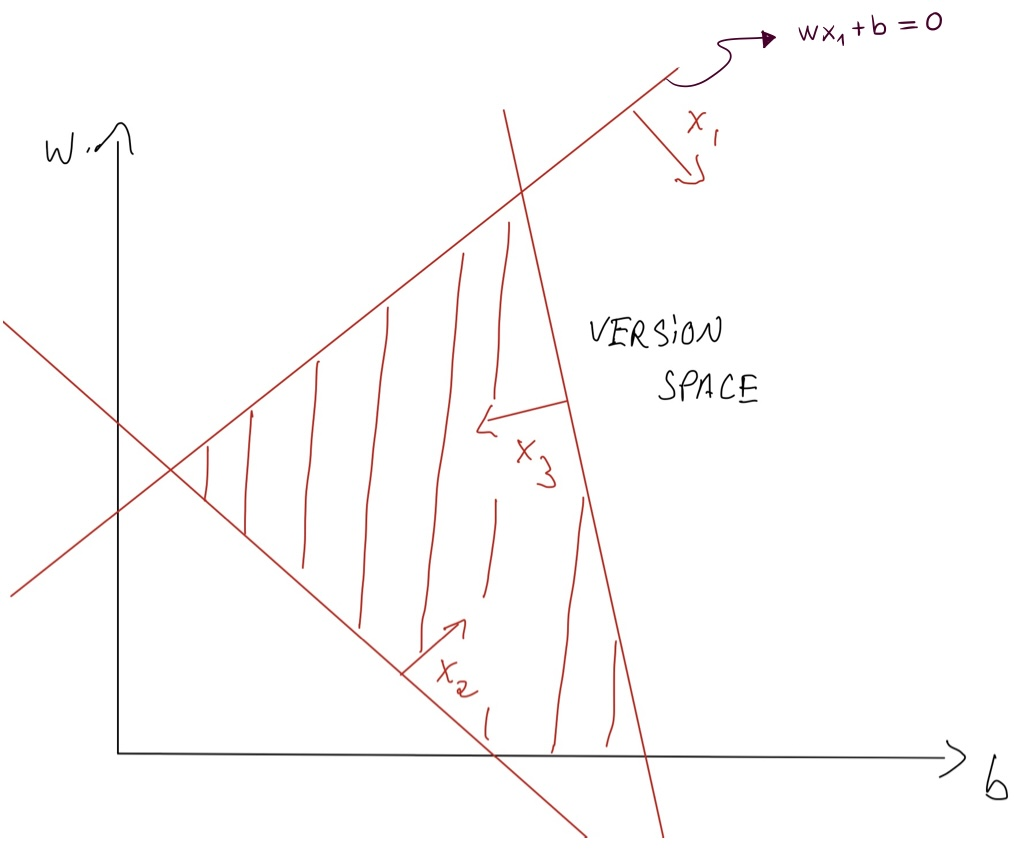
\includegraphics[scale = 0.05]{contents/imgs/versionspace.jpeg}
%\end{center}


\textbf{Linear Separability:} The version space of a linear threshold classifier is $\mathcal{V}(\mathcal{S}) = \{(w, b): \gamma[w, b](\mathcal{S}) > 0 \}\subseteq \mathbb{R}^{n + 1}$. We call $\mathcal{S}$ linearly separable if and only if $\mathcal{V}(\mathcal{S}) \neq \emptyset$ ($\implies$ perceptron learning aims to find a perfect linear separator, and does not explicitly aim (and is not guaranteed) to find classifier with low training error).


\textbf{Perceptron Learning:} 
\begin{itemize}
    \item Present training examples repeatedly in some arbitrary order, making sure every example is repeated after finite number of steps.
    \item Follow the update rule: $f[w, b](x) \neq y \implies w\leftarrow w + yx, \quad b \leftarrow b + y$. Note how the perceptron only learns from mistakes!
\end{itemize}  


\textbf{Perceptron weights:} $w^0 \in span(x_1, \dots, x_s) \implies w^t \in span(x_1, \dots, x_s), \ \forall t $


\textbf{Convergence:} General setting: Set $b=0$, initialize $w^0=0$. 
\begin{itemize}
    \item \textbf{Lemma} Let $w, \ \lVert w\rVert = 1,$ such that $\gamma[w](\mathcal{S}) = \gamma > 0$. Then $w^t \cdot w \geq t\gamma$. 
    \item \textbf{Lemma} Let $R =max_{x\in \mathcal{S}}\ \lVert x\rVert$, then $\lVert w^t \rVert \leq R \sqrt{t}$
    \item \textbf{Theorem} Let $\mathcal{S}$ be $\gamma$-separable, $R = max_{x \in \mathcal{S}}\ \lVert x\rVert$. The perceptron converges in at most $\lfloor R^2 / \gamma ^2\rfloor$ steps.
    \item \textbf{Exercise} Let $(x^t, y^t)$ be sequence of mistakes, inducing updates $\Delta\theta^t$, $\theta^s=\sum_{t = 1}^s \Delta\theta^t$. Then $\lVert\theta^s\lVert^2 \leq\sum_{t =1}^s \lVert x^t\rVert^2$.
\end{itemize}


\textbf{Combinatorics and Geometry:} General setting: Set $b = 0$.
\begin{itemize}
    \item \textbf{Number of ways} to classify $s$ points in $n$-space with linear classifier: $C(\mathcal{S}, n) = |\{y \in \{-1, 1\}^s\ | \ \exists w \in \mathbb{R}^n: \ \forall(x, y) \in \mathcal{S} : \ y(x \cdot w) > 0\}|$
    \item \textbf{General position:} $\mathcal{X}=\{x_1, \dots, x_s\} \subset \mathcal{R}^n$ are in general position if and only if $\forall \Xi \subseteq \mathcal{X}$ with $|\Xi| \leq n: \ \Xi$ is linearly independent.
    \item \textbf{Cover's Theorem:} Let $\mathcal{S} \subset \mathbb{R}^n$ be a set of $s$ points in general position. Then $C(s + 1, n) = 2 \sum_{i = 0}^{n-1} {s \choose i}$
    \item \textbf{Corollary:} $C(s, n) = 2^s$ for $s \leq n$.
    \item \textbf{Asymptotic Shattering:} 
        $\frac{C(s,n)}{2^s} \;=\;
        \begin{cases}
          1 & \text{if } s \le n,\\
          1 \;-\; \mathcal{O}(e^{-n}) & \text{if } n < s < 2n,\\
          \tfrac12 & \text{if } s = 2n,\\
          \mathcal{O}(e^{-n}) & \text{otherwise}.
        \end{cases}$
    \item \textbf{Interpretation:} There two growth regimes. One where the number of realizable labelings grows exponentially, and one where the growth function of realizable labelings starts go get constrained by geometry.
\end{itemize}

\subsection{Parallel Distributed Processing}

%
%\textbf{Elements:} \begin{enumerate}
%    \item A set of processing units with states of activation
%    \item Output functions for each unit
%    \item A pattern of connectivity between units
%    \item Propagation rules for propagating patterns of activity
%    \item Activation functions for units
%    \item Learning rule to modify connectivity based on experience (train data)
%    \item An environment within which the system operates (e.g. loss function)
%\end{enumerate}


\textbf{Layers and Activation Functions:} The layer transfer function is $f(W,B)(x) = \Phi(Wx +B), \; W= (w_1, \dots, w_m)^{\intercal}, \;\Phi(z)=(\phi(z_1), \dots, \phi(z_m))^{\intercal}$. Note how the linear threshold unit is a special case with $\phi = \text{sign}$. 


\textbf{Delta Rule:}
\begin{itemize}
    \item The original perceptron update rule has disadvantages:
    \begin{itemize}
        \item $0/1$ classification error not differentiable at decision boundary and has zero derivatives elsewhere.
        \item We do not learn anything from correctly classified points.
    \end{itemize}
    \item The delta learning rule can be formulated as follows:  \\$\Delta w_{i,j}=\eta\delta_i\phi'(w_i \cdot x)x_j, \; \delta_i=(y_i - f_i), \; \eta > 0$
\end{itemize}


\textbf{Remarks:} \begin{itemize}
    \item Update of a weight vec. for a unit is always in dir. of a training point
    \item The update is scaled by the residual (or delta) $\delta_i$ of the unit
    \item The \emph{sensitivity} of the unit factors in (derivative of activation)
    \item $\eta$ is a design choice
    \item The delta rule is nothing but a gradient step with step size $\eta$, i.e., $\Delta w_{i, j} = -\eta \frac{\partial \ell}{\partial w_{i,j}}$ with squared loss $\ell = \frac{1}{2} \sum_{i = 1}^{m} (\phi_i - y_i)^2$
    \item Generalized delta rule for deep architectures: $\delta_i = \frac{\partial \ell}{\partial \phi_i}$, derived by propagating error terms from the outputs back towards the inputs
\end{itemize}


\textbf{Multi-Layer Perceptron:} Particular neural network architecture that can be written as (for $n$ inputs, $m$ hidden units, and one real output): $f[v, W](x) = \sum_{i = 1}^m v_i\phi_i, \; \phi_i = \phi(w_i \cdot x), \; \phi(z) = \frac{1}{1 + e^{-z}}$. 

\subsection{Hopfield Networks: Classical model of an associate memory} 

\textbf{Idea:} Define a parameterized energy function via
second order interaction of $n$ binary neurons: \\ $E(X) = -\frac{1}{2}\sum_{i \neq j} w_{i,j}X_iX_j + \sum_i b_i X_i, \; X_i \in \{-1, +1\}, \; 1 \leq i \leq n$. \\ Where we constrain the weights as follows: $w_{i,j} = w_{j, i} \;(\forall i, j), \; w_{i, i} = 0\; (\forall i)$. Think of the weights as quantifying the interaction strength between neurons, and of the biases as thresholds (set to zero in the following).


\textbf{Dynamics:} After initialization, the state of each neuron is iteratively (in some fixed order) updated as follows: $X_i \leftarrow \begin{cases}
    +1 \; \text{if}\; E(\dots, X_{i-1}, +1, X_{i+1}, \dots) \leq E(\dots, X_{i-1}, -1, X_{i+1}, \dots) \\
    -1 \; \text{else}
\end{cases}$, where updates can be performed synchronous or asynchronous. \textbf{Note} that asynchronous updates guarantee that the energy function will never increase. \textbf{Note} after a finite number of steps, a fixed point is reached, which is the pattern of the Hopfield network.


\textbf{Simplified update Rule:} Instead of evaluating the $n(n+1)/2$ summands in $E$, we can just calculate $n$ terms: $H_i =\sum_j w_{i,j} X_j$ and follow the update rule $X_i=\text{sign}(H_i)$. Here $\text{sign}(0) = 1$.


\textbf{Hebbian Learning:} Given a set $\mathcal{S}$ with patterns $x^t \in \{\pm1\}^n, \; (1\leq t \leq s)$. Then choose the weights as $w_{i,j} = \frac{1}{n}\sum_{t = 1}^s x_i^tx_j^t$, which in matrix notation can be written as $W = \frac{1}{n} \sum_{t = 1}^s x^t x^{t^{\intercal}}$ ($\implies$ neurons that fire together wire together)


\textbf{Memorization:} For a pattern to be included in associative memory, the pattern must define a meta-stable state: $x_i^t = \text{sign}\big(\sum_{j = 1}^n w_{i,j} x_j^t\big)$ (the dynamics will not diverge from the pattern).


\textbf{Cross-talk term between patterns:} Using the couplings learned with Hebbian learning, we get: $\sum_{j = 1}^n w_{i,j} x_j^t = x_i^t + \frac{1}{n} \sum_{j = 1}^n \sum_{r \neq t} x_i^r x_j^r x_j^t$, where $C_i^t = \frac{1}{n} \sum_{j = 1}^n \sum_{r \neq t} x_i^r x_j^r x_j^t$ is called the cross-talk between patterns. \textbf{For $x^t$ to be stable, we require this term to be strictly less than 1 in magnitude for all neurons.} 


\textbf{Capacity:} Assume patterns to be random signs (probability of $\frac{1}{2}$ for $-1$ and $+1$). Assume that $n\rightarrow \infty$. Then $C_i^t \overset{\text{approx.}}{\sim}\mathcal{N}(0, \frac{s}{n})$. Then the error probability of any sign to be incorrectly flipped becomes: $P_e = \text{Prob}\{-x_i^tC_i^t\}\approx \int_1^\infty e^{-\frac{nz^2}{2s}}dz=\frac{1}{2}\big[1 - \text{erf}(\sqrt{n/2s})\big]$ ($\implies$ ratio $s/n$ controls asympt. err. rate).


$\implies$ It can be shown that a phase transition occurs at $s/n \approx0.138$. Beyond that limit many errors occur. If one requires that a pattern is retrieved with high probability, then one gets a sub-linear capacity bound of $s\leq \frac{n}{2 \text{log}_2n}$\\
\textbf{Spurious patterns:} Simplest spurious pattern: sign inverted version of stable pattern is also stable as the network is sign symmetric.




